\documentclass[a4paper,14pt]{article}
\usepackage[utf8]{inputenc}  %% 1
\usepackage[T2A]{fontenc}      %% 2
\usepackage[english,russian]{babel}    %% 3
\usepackage{amssymb, amsmath,mathtext,cite,enumerate,float}
\usepackage{helvet}
\usepackage{matlab-prettifier}
\usepackage{graphicx}

\parindent=1.25cm

\newcommand*{\No}{\textnumero}

\begin{document}

\begin{titlepage}
\newpage

\begin{center}
Санкт-Петербургский государственный политехнический университет \\
\end{center}

\begin{center}
Институт прикладной математики и механики \\ 
\end{center}

\begin{center}
\textbf{Кафедра "Прикладная математика и информатика"} \\ 
\end{center}

\vspace{2em}

\begin{center}
\LARGE{\textbf{Отчет по лабоработрной работе 1}}
\end{center}

\vspace{14em}


\begin{center}
Санкт-Петербург \\2018
\end{center}

\end{titlepage}

\section{Постановка задачи}

Ознакомиться с пакетными реализациями наивного Байесовского классификатора и их использованием, проследив, как объемы тестовой и обучающей выборок влияют на качество классификации. Проиллюстрировать свои выводы графиками. В качестве материалов использовать предоставленные наборы данных.

\section{Используемые функции}

В данной работе использовалась реализация наивного Байесовского классификатора из пакета scikit-learn для языка Python. Пример использования приведен в листинге \ref{lst:usage}

\begin{lstlisting}[caption={Использование байесовского классификатора из пакета scikit-learn}, label={lst:usage}, language=Python]
from sklearn.naive_bayes import GaussianNB
gnb = GaussianNB()
y_pred = gnb.fit(x, y).predict(x)
\end{lstlisting}

\textbf{Аргументы и возвращаемые значения:}
\begin{itemize}
	\item функции fit(x, y):\\ x - матрица данных; y - вектор меток классов. Возвращает экземпляр классификатора, обученный на соответсвующих данных
	\item функции predict(x): \\ x - матрица данных. Возвращает вектор предсказанных меток.
\end{itemize}

\section{Проделанная работа}

\subsection{Задание 1}

\textbf{Постановка задачи:}

Исследуйте, как объем обучающей выборки и количество тестовых данных, влияет на точность классификации или на вероятность ошибочной классификации в примере крестики-нолики и примере о спаме e-mail сообщений.\\

Для вычислений использовалась фунция evaluate, код которой приведен в листинге \ref{lst:sizes}.

\begin{lstlisting}[caption={Использование байесовского классификатора из пакета scikit-learn}, label={lst:sizes}, language=Python]
def evaluate(data, sizes, clf_constructor):
	acc = list()
	dataset = shuffle(data)

	for i in train_size:
		clf = clf_constructor()
		clf.fit(dataset[dataset.columns[:-1]][:i],
			dataset[dataset.columns[-1]][:i])
		acc.append(clf.score(dataset[dataset.columns[:-1]][i:],
			dataset[dataset.columns[-1]][i:]))

	return acc
\end{lstlisting}

\textbf{Аргументы и возвращаемые значения:}
\begin{itemize}
	\item {[in]} data - данные для обработки;
	\item {[in]} sizes - проверяемые размеры обучающей выборки. Не вошедшие в обучающую выборку данные становятся тестовыми;
	\item {[in]} clf\_constructor - конструктор исследуемого классификатора;
	\item {[out]} acc - результаты вычислений.
\end{itemize}

Результаты вычислений для датасета Tic\_tac\_toe приведены на рис. \ref{graph:tic_acc}, для датасета со спамом - на рис. \ref{graph:spam_acc}.

\begin{figure}[H]
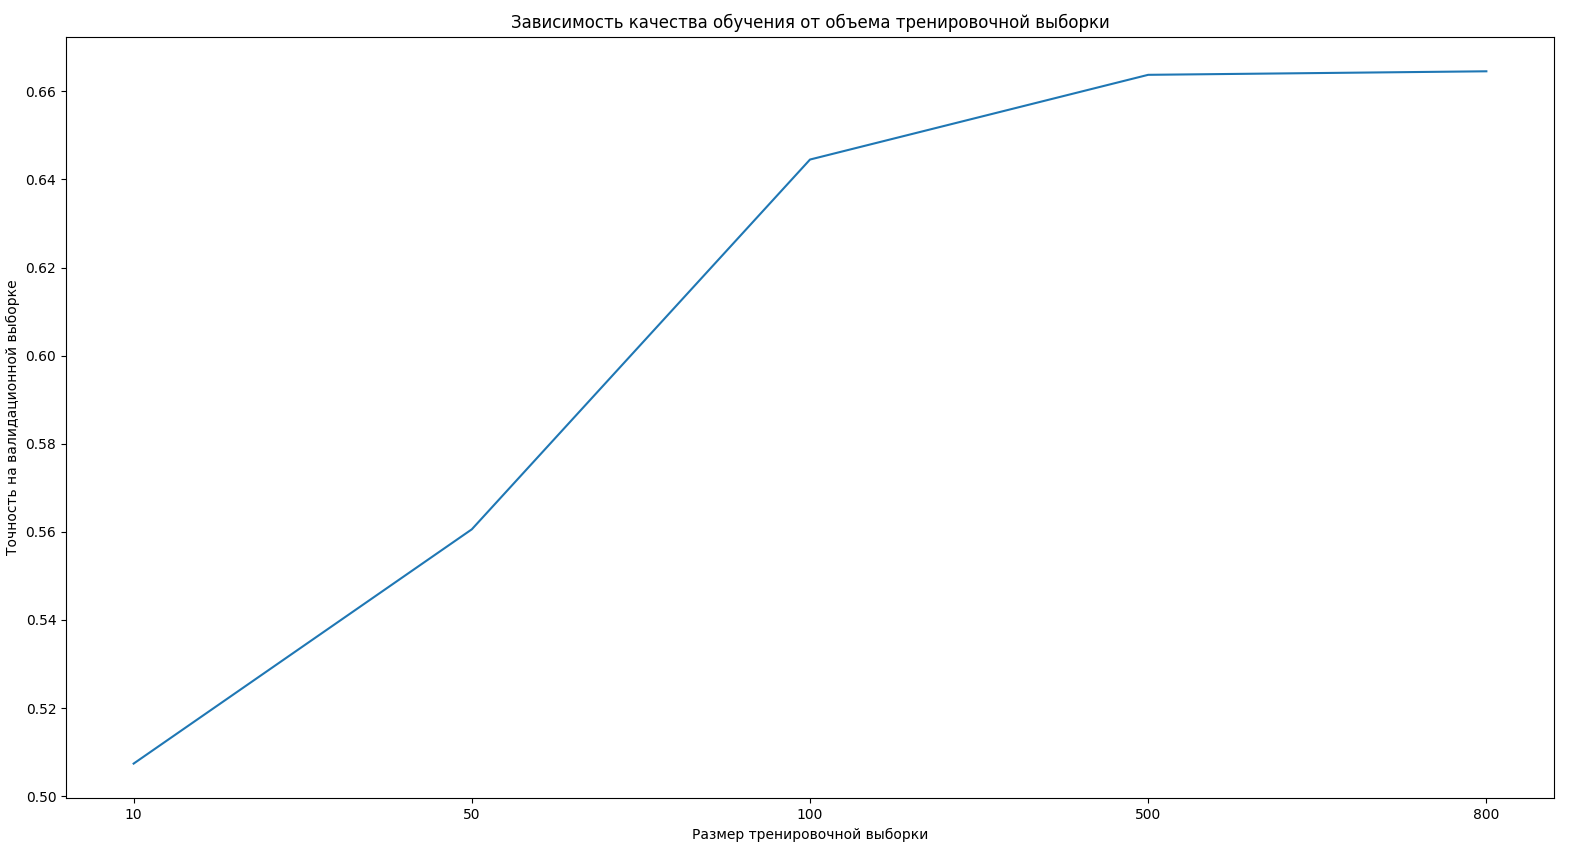
\includegraphics[width=\textwidth, keepaspectratio]{tic_acc.png}
\caption{Зависимость точности обучения об объема обучающей выборки для датасета tic\_tac\_toe}
\label{graph:tic_acc}
\end{figure}

\begin{figure}[H]
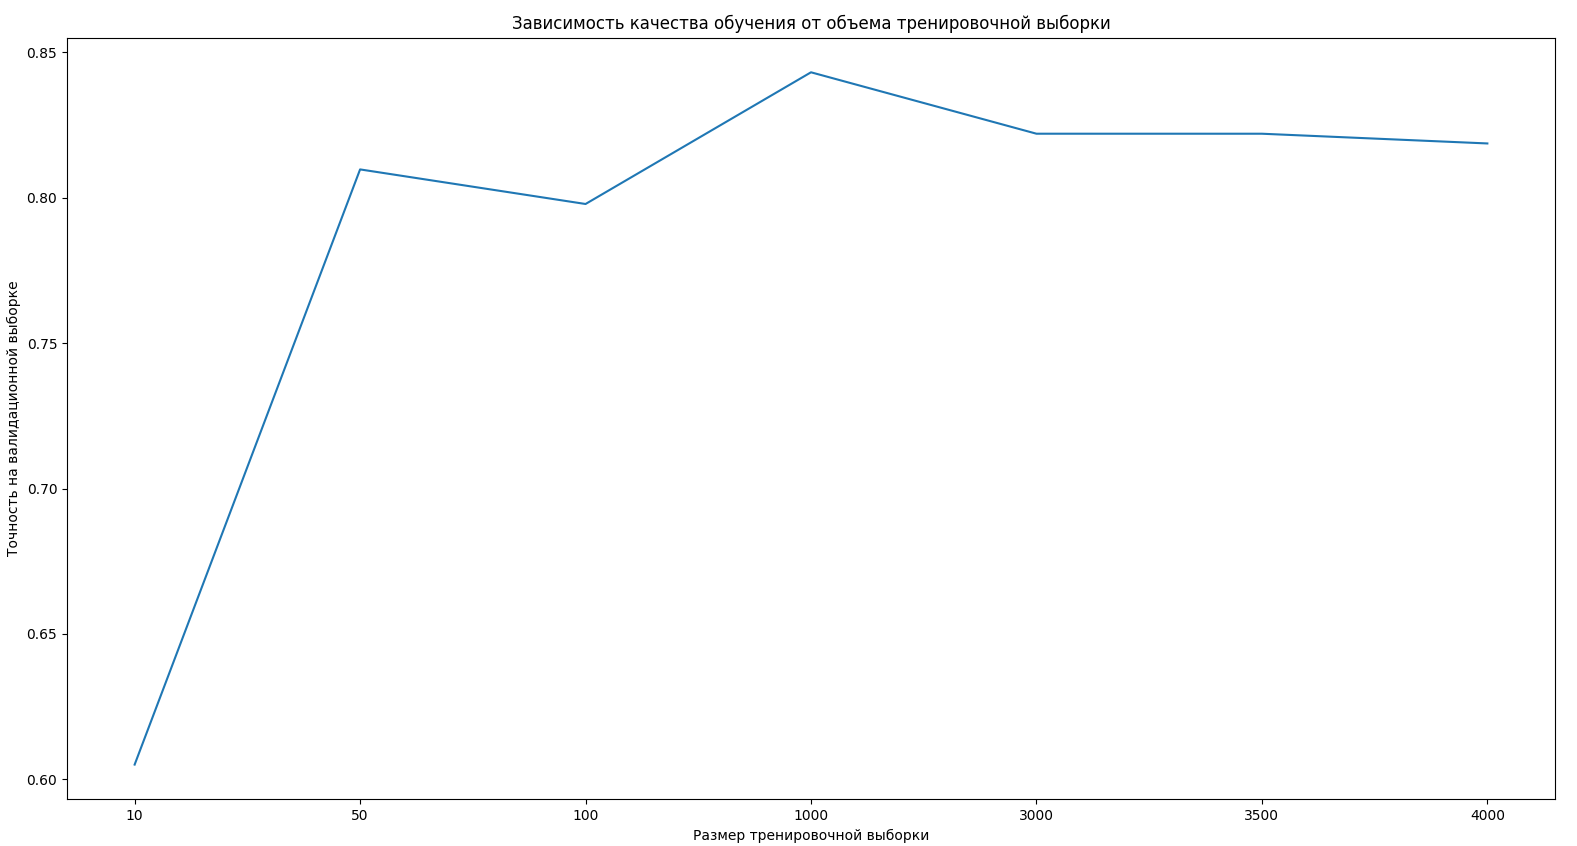
\includegraphics[width=\textwidth, keepaspectratio]{spam_acc.png}
\caption{Зависимость точности обучения об объема обучающей выборки для датасета spambase}
\label{graph:spam_acc}
\end{figure}


\subsection{Задание 2}

\textbf{Постановка задачи:}
Сгенерируйте 100 точек с двумя признаками X1 и X2 в соответствии с нормальным распределением так, что первые 50 точек (class -1) имеют параметры: мат. ожидание X1  равно 10, мат. ожидание X2 равно 14, среднеквадратические отклонения для обеих переменных равны 4. Вторые 50 точек (class +1) имеют параметры: мат. ожидание X1 равно 20, мат. ожидание X2 равно 18, среднеквадратические отклонения для обеих переменных равны 3. Построить соответствующие диаграммы, иллюстрирующие данные. Построить байесовский классификатор и оценить качество классификации. \\

\textbf{Результаты:}

Распределение сгенерированных с помощью функции multivariate\_normal модуля random пакета numpy данных приведено на рис. \ref{graph:task_2}. Точность гауссовского наивного байесовского классификатора, протестированного на 10 примерах из сгенерированной выборки, составила 94\%.
\begin{figure}[H]
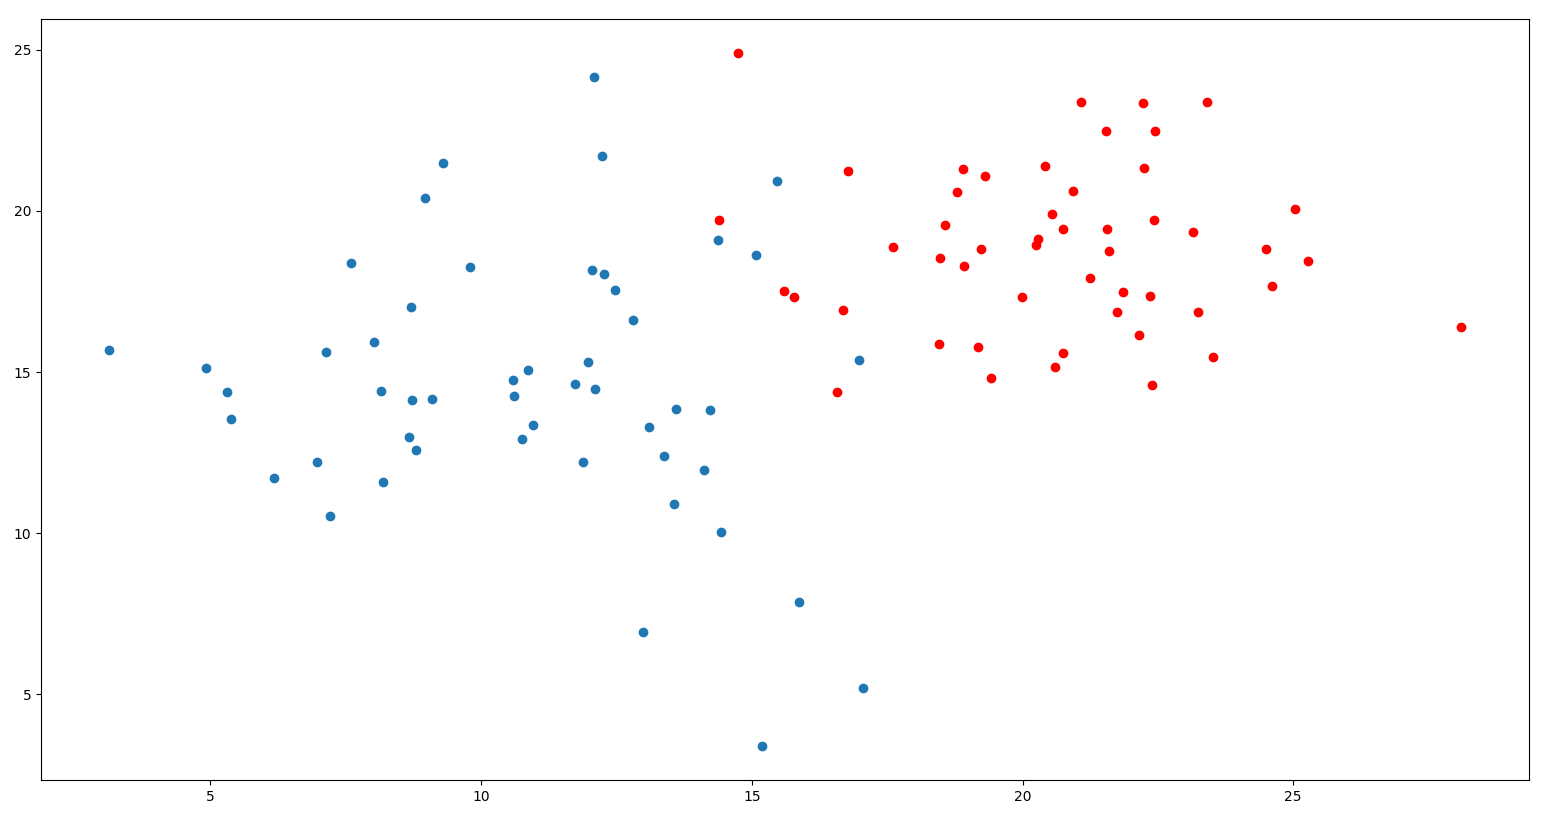
\includegraphics[width=\textwidth, keepaspectratio]{task_2.png}
\caption{Распределение сгенерированных данных}
\label{graph:task_2}
\end{figure}

\subsection{Задание 3}

\textbf{Постановка задачи:}
Разработать байесовский классификатор для данных Титаник (Titanic dataset) 

\textbf{Результаты:}

Функция prepare\_dataset, выполняющая предобработку входных данных, приведена в листинге \ref{lst:preprocess}.

\textbf{Аргументы и возвращаемые значения:}
\begin{itemize}
	\item {[in]} filename - путь к файлу с данными;
	\item {[in]} to\_drop - колонки, которые не несут ценной информации;
	\item {[in]} to\_factorize - колонки, значения которых нужно заменить числовыми вместо строковых;
	\item {[in]} to\_fill - колонки, содержащие пропуски;
	\item {[out]} dataset - предобработанный датасет.
\end{itemize}


\begin{lstlisting}[caption={Чтение и предобработка входных данных}, label={lst:preprocess}, language=Python, breakatwhitespace=true, tabsize=2]
def prepare_dataset(filename, to_drop=None, to_factorize=None, to_fill=None):
	with open(filename) as f:
		dataset = pd.read_csv(f, sep=',')

	dataset = dataset.drop(to_drop, axis=1)

	#convert string features to numbers
	for column in to_factorize:
		dataset[column] = pd.factorize(dataset[column])[0]

	imp = SimpleImputer(missing_values=np.nan, strategy='mean')

	for column in to_fill:
		column_reshaped = [[el] for el in dataset[column]]
		to_transofrm = [[el] for el in dataset[column]]
		dataset[column] = imp.fit(column_reshaped).transform(to_transform)

	return dataset
\end{lstlisting}

В случае датасета Titanic колонки 'PassengerId', 'Cabin', 'Ticket' явно не несут в себе ценной информации, поскольку их значения уникальны для каждого пассажира. Значения в колонках 'Sex', 'Embarked' были представлены строковыми переменными, поэтому нуждались в факторизации. Поле 'Age' содержало пропуски, заполненные средним для остального датасета значениями.

Полученный с учетом этих соображений код для построения и тестирования классификатора приведен в листинге \ref{lst:titanic}. Его точность на тестовом наборе размером 67 составила 79\%.

\begin{lstlisting}[caption={Построение классификатора для датасета Titanic}, label={lst:titanic}, language=Python]
dataset = prepare_dataset('../Titanic_train.csv',
	to_drop=['PassengerId', 'Cabin', 'Ticket'],
	to_factorize=['Sex', 'Embarked'],
	to_fill=['Age'])

clf = nb.GaussianNB()
clf.fit(dataset.drop('Survived', axis=1).values[:train_size], 
	list(dataset['Survived'])[:train_size])

acc = clf.score(dataset.drop('Survived', axis=1).values[train_size:], 
	list(dataset['Survived'])[train_size:])
\end{lstlisting}






\end{document}